\section*{مقدمه}
\lr{cuckoo sandbox} یک ابزار \lr{open source} برای تحلیل خودکار بدافزار ها می باشد و این امکان را فراهم می‌سازد که فایل‌های مشکوک در یک محیط مجازی اجرا شده و رفتار آن‌ها از جمله فعالیت‌های فایل، ارتباطات شبکه‌ای، و تغییرات در رجیستر ها مورد بررسی قرار گیرد. این ابزار نقش مهمی در شناسایی تهدیدات سایبری و پاسخ به حوادث امنیتی ایفا می‌کند. در این گزارش، مراحل راه‌اندازی \lr{Cuckoo}، کاربردهای عملی آن، و نحوه تعامل با \lr{API}ها به‌صورت جامع مورد بررسی قرار گرفته است.
\section*{بخش اول: نصب و راه اندازی}
\subsection*{تلاش اول: دو ماشین مجازی تو در تو}
در ابتدا نسخه \lr{22.04} توزیع \lr{Ubuntu} لینوکس را روی ماشین مجازی نصب کرده و \lr{windows7} را روی یک ماشین مجازی دیگر داخل آن به صورت تو در تو نصب کردیم. تعدادی از مراحل نصب \lr{Cuckoo} در این روش انجام شدند اما به دلیل مشکلات هنگام نصب و عدم بوت شدن سیستم عامل علا رغم تلاش برای \lr{toubleshooting} روش دیگری را نصب ابزار انتخاب کردیم و مراحل نصب را مجددا از ابتدا آغاز کردیم.
\subsection*{تلاش دوم: نصب مستقیم لینوکس روی سیستم}
برای نصب \lr{Cuckoo} نیاز به یک سیستم عامل میزبان (\lr{Ubuntu22.04}) و یک سیستم عامل مهمان (\lr{windows7}) داشتیم که روی ماشین مجازی \lr{KVM} نصب شد. هم چنین سایر \lr{dependency} های دو سیستم عامل روی آن ها نضب شده و \lr{configuration} های مورد نیاز انجام شدند. در ادامه همه مراحل به تفصیل توضیح داده خواهند شد: 
\subsection*{آماده سازی میزبان}
\subsubsection*{نصب سیستم عامل:}
ابتدا سیستم عامل \lr{Ubuntu 22.04} را به دلیل سازگاری بیشتر با \lr{cuckoo} مستقیما روی سیستم نصب کردیم. (به صورت \lr{dual boot})
\subsubsection*{نیازمندی ها:}
\begin{enumerate}
    \item پایتون و کتابخانه های مورد نیاز آن را روی \lr{Ubuntu} نصب کردیم. نکته مهم در این قسمت استفاده از ورژن \lr{python 2.7} بود که توسط \lr{cuckoo} ساپورت می شود.
    تصاویر زیر مراحل انجام این این و خطاهای رخ داده را نشان می دهند:
    \begin{figure}[htbp]
      \centering
      \includegraphics[width=0.8\textwidth]{Template - Student/Content/screenshots/Screenshot from 2025-04-17 21-22-05}
      \caption{First Image}
      \label{fig:vert1}
    \end{figure}
    
    \begin{figure}[htbp]
      \centering
      \includegraphics[width=0.8\textwidth]{Template - Student/Content/screenshots/Screenshot from 2025-04-17 21-22-29}
      \caption{Second Image}
      \label{fig:vert2}
    \end{figure}
    \begin{figure}[htbp]
      \centering
      \includegraphics[width=0.8\textwidth]{Template - Student/Content/screenshots/Screenshot from 2025-04-17 21-22-29}
      \caption{Second Image}
      \label{fig:vert2}
    \end{figure}
    \begin{figure}[htbp]
      \centering
      \includegraphics[width=0.8\textwidth]{Template - Student/Content/screenshots/Screenshot from 2025-04-17 21-22-52}
      \caption{Second Image}
      \label{fig:vert2}
    \end{figure}
    \begin{figure}[htbp]
      \centering
      \includegraphics[width=0.8\textwidth]{Template - Student/Content/screenshots/Screenshot from 2025-04-17 21-23-03}
      \caption{Second Image}
      \label{fig:vert2}
    \end{figure}
    \begin{figure}[htbp]
      \centering
      \includegraphics[width=0.8\textwidth]{Template - Student/Content/screenshots/Screenshot from 2025-04-17 21-23-24}
      \caption{Second Image}
      \label{fig:vert2}
    \end{figure}
    \begin{figure}[htbp]
      \centering
      \includegraphics[width=0.8\textwidth]{Template - Student/Content/screenshots/Screenshot from 2025-04-17 21-23-39}
      \caption{Second Image}
      \label{fig:vert2}
    \end{figure}
    \item یک محیط مجازی برای نصب \lr{cuckoo} ایجاد کردیم.
    \begin{figure}[]
      \centering
      \includegraphics[width=0.8\textwidth]{Template - Student/Content/screenshots/Screenshot from 2025-04-17 21-23-56}
      \caption{Second Image}
      \label{fig:vert2}
    \end{figure}
    \item \lr{mongodb} را روی سیستم نصب کردیم.
    \begin{figure}[htbp]
      \centering
      \includegraphics[width=0.8\textwidth]{Template - Student/Content/screenshots/Screenshot from 2025-04-17 21-23-56}
      \caption{Second Image}
      \label{fig:vert2}
    \end{figure}
    \item \lr{postgresql} را روی سیستم نصب کردیم.
    \begin{figure}[htbp]
      \centering
      \includegraphics[width=0.8\textwidth]{Template - Student/Content/screenshots/Screenshot from 2025-04-17 21-24-56}
      \caption{Second Image}
      \label{fig:vert2}
    \end{figure}
    \item ابزار \lr{tcpdump} را روی سیستم نصب کردیم.
    \begin{figure}[htbp]
      \centering
      \includegraphics[width=0.8\textwidth]{Template - Student/Content/screenshots/Screenshot from 2025-04-17 21-26-27}
      \caption{Second Image}
      \label{fig:vert2}
    \end{figure}
    \item یک \lr{user} به نام \lr{cuckoo} در \lr{Ubuntu} ایجاد کردیم و گروه و دسترسی های لازم را به آن دادیم و پسورد آن را غیرفعال کردیم تا بتوانیم با استفاده از آن با ابزار \lr{cuckoo} کار کنیم.
    \begin{figure}[htbp]
      \centering
      \includegraphics[width=0.8\textwidth]{Template - Student/Content/screenshots/Screenshot from 2025-04-17 21-26-27}
      \caption{Second Image}
      \label{fig:vert2}
    \end{figure}
\end{enumerate}
\subsubsection*{نصب \lr{cuckoo}:}
در این مرحله ابزار \lr{cuckoo} را در محیط مجازی که برای آن ساخته شده بود و \lr{cuckoo user} نصب کرده و اجرای آن را بررسی کردیم. 
\begin{figure}[htbp]
      \centering
      \includegraphics[width=0.8\textwidth]{Template - Student/Content/screenshots/Screenshot from 2025-04-17 21-26-34}
      \caption{Second Image}
      \label{fig:vert2}
    \end{figure}
    \begin{figure}[htbp]
      \centering
      \includegraphics[width=0.8\textwidth]{Template - Student/Content/screenshots/Screenshot from 2025-04-17 21-26-54}
      \caption{Second Image}
      \label{fig:vert2}
    \end{figure}
\subsubsection*{\lr{virtualization}:}
برای کار با ابزار \lr{cuckoo} در این پروژه نیاز به یک سیستم عامل مهمان (\lr{windows7}) داشتیم که روی یک ماشین مجازی روی سیستم عامل میزبان نصب شود تا فایل هایی که برای تحلیل به ابزار می دهیم داخل آن اجرا شوند.
\begin{enumerate}
    \item برای این کار ابتدا از نرم افزار \lr{virtualbox} برای \lr{virtualization} استفاده کردیم. این ابزار با استفاده از دستور زیر نصب کردیم:
    \begin{figure}[htbp]
      \centering
      \includegraphics[width=0.8\textwidth]{Template - Student/Content/screenshots/Screenshot from 2025-04-17 21-25-51}
      \caption{Second Image}
      \label{fig:vert2}
    \end{figure}
    و بعد \lr{windows7} را روی آن نصب کردیم. تصاویر زیر تعدادی از مراحل نصب را نشان می دهند.
    \begin{figure}[htbp]
      \centering
      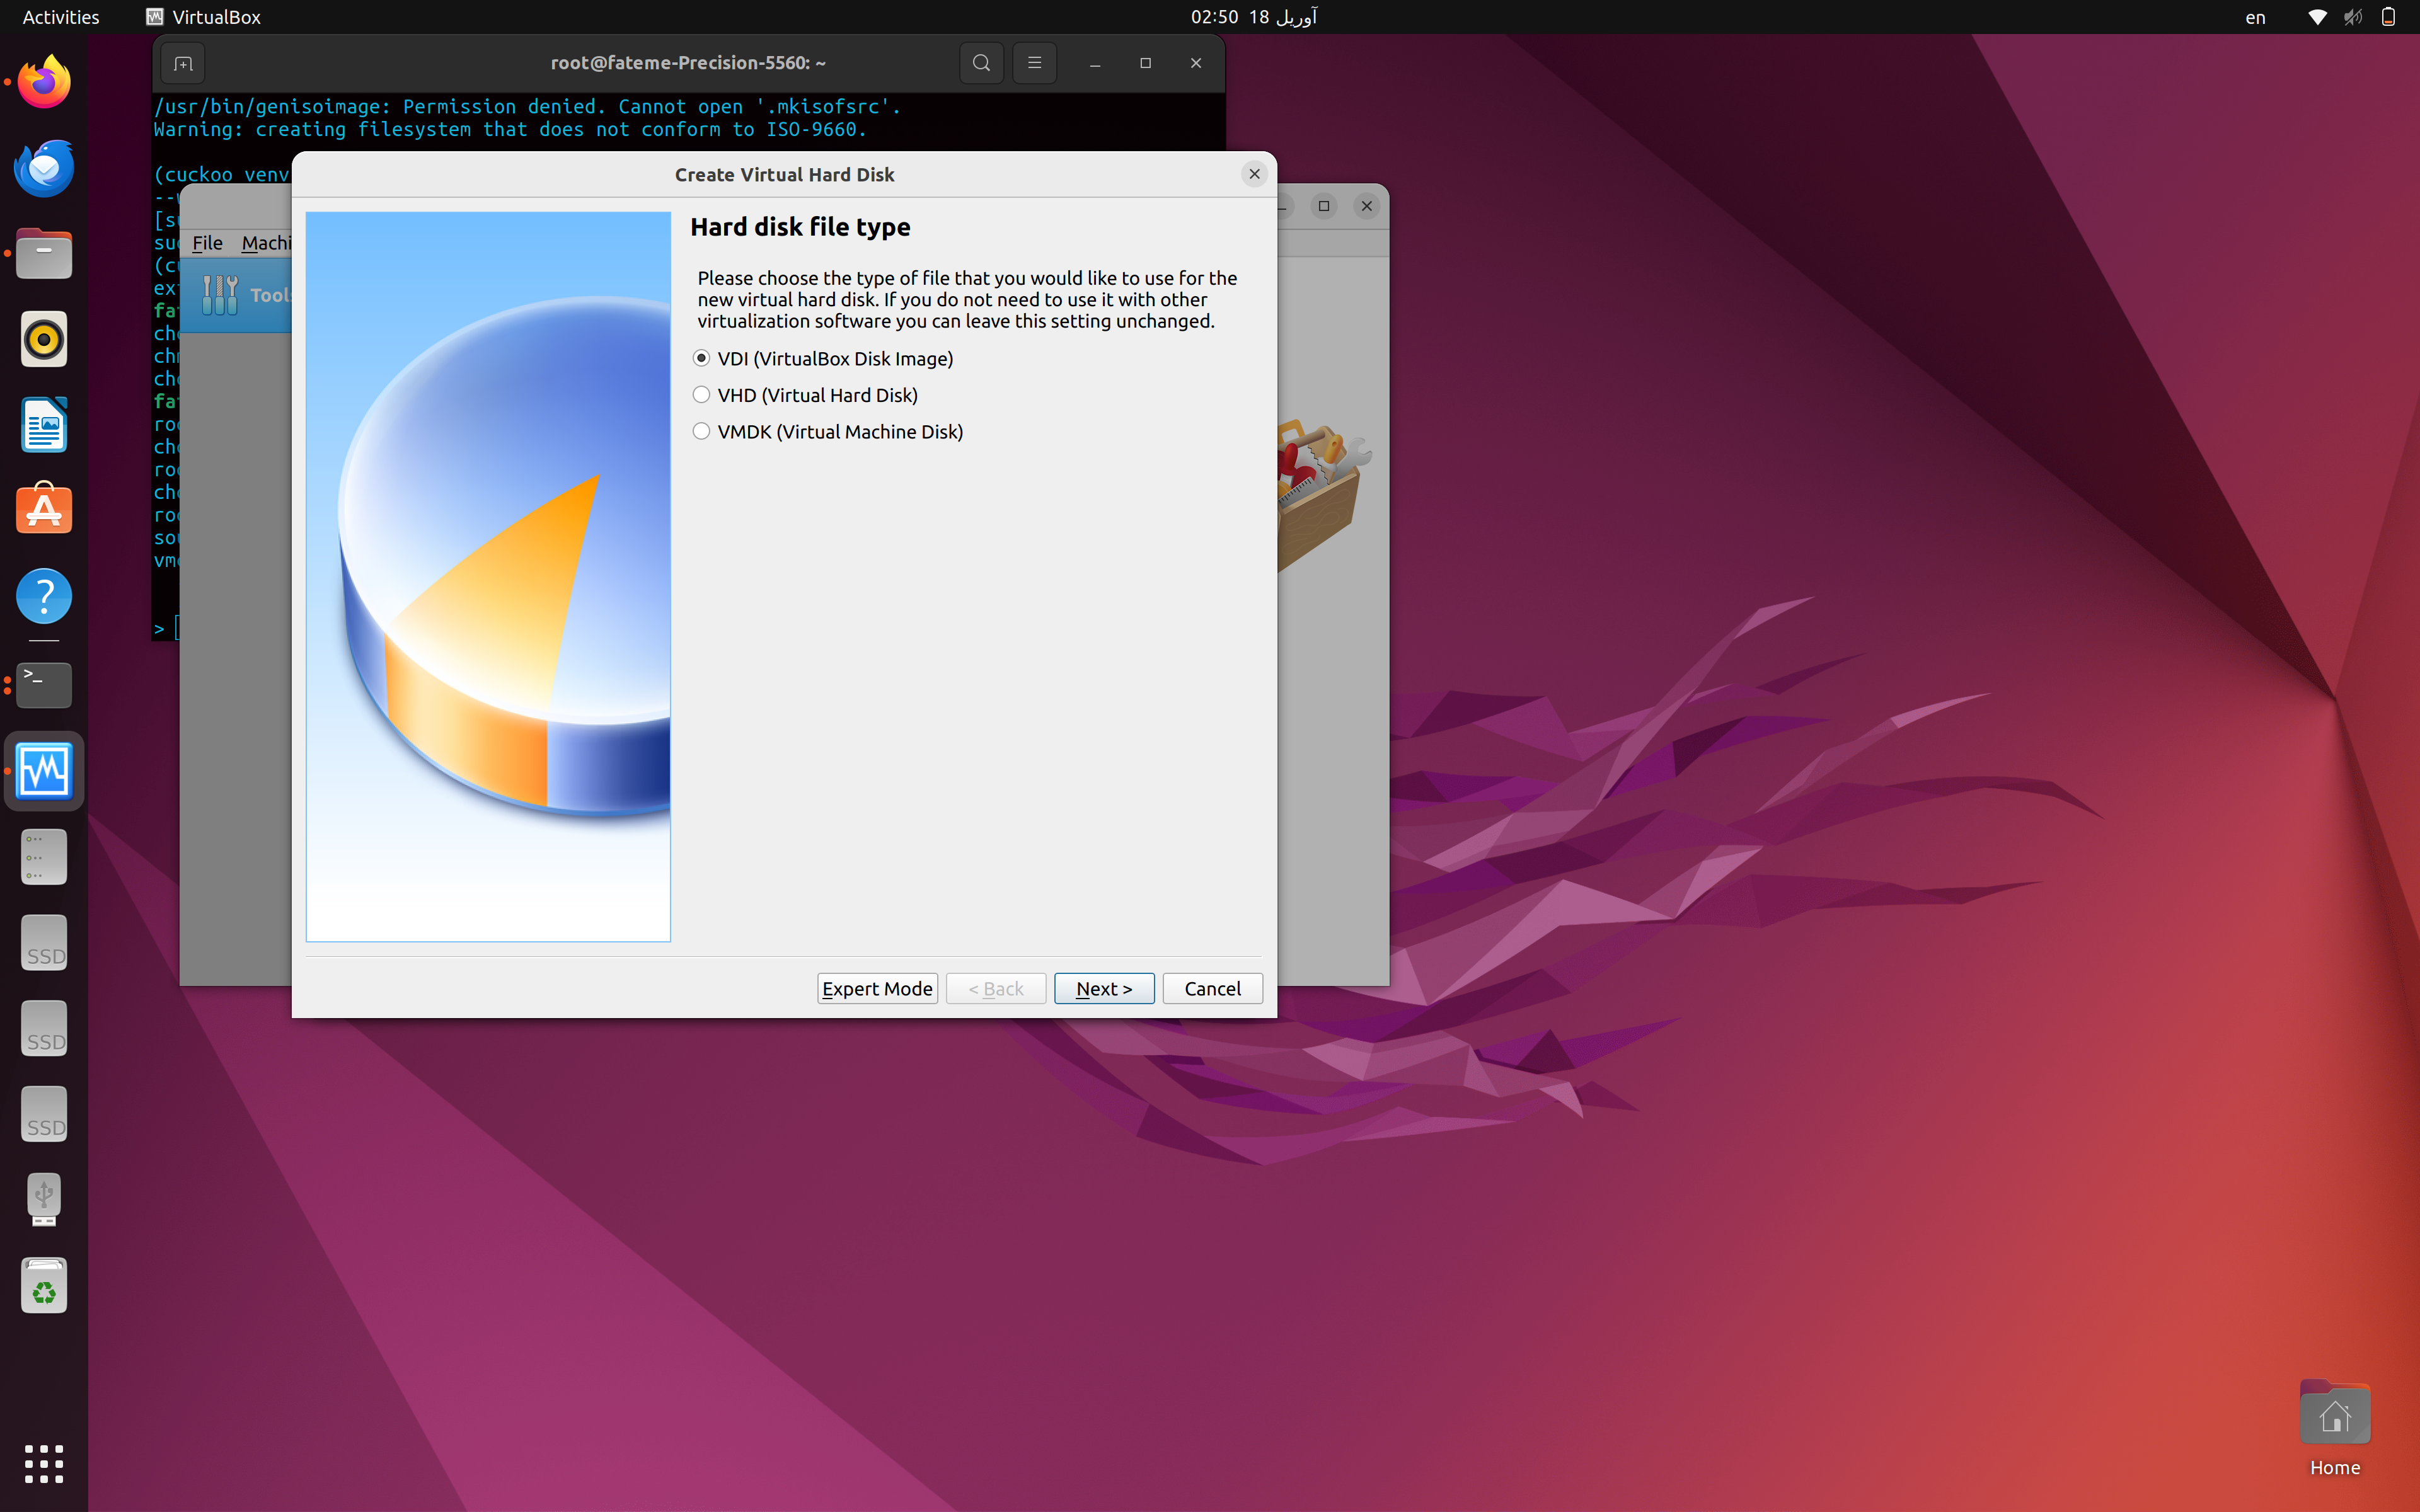
\includegraphics[width=0.8\textwidth]{Template - Student/Content/screenshots/Screenshot from 2025-04-18 02-50-20}
      \caption{Second Image}
      \label{fig:vert2}
    \end{figure}
    \begin{figure}[htbp]
      \centering
      \includegraphics[width=0.8\textwidth]{Template - Student/Content/screenshots/Screenshot from 2025-04-17 03-50-13}
      \caption{Second Image}
      \label{fig:vert2}
    \end{figure}
    \begin{figure}[htbp]
      \centering
      \includegraphics[width=0.8\textwidth]{Template - Student/Content/screenshots/Screenshot from 2025-04-17 04-08-04}
      \caption{Second Image}
      \label{fig:vert2}
    \end{figure}
    تصاویر زیر خطای رخ داده بعد از نصب \lr{windows} و تعدادی از تلاش های انجام شده برای حل مشکل (از جمله نصب مجدد ویندوز با استفاده از \lr{command line}) را نشان می دهند:
    \begin{figure}[htbp]
      \centering
      \includegraphics[width=0.8\textwidth]{Template - Student/Content/screenshots/Screenshot from 2025-04-17 04-09-21}
      \caption{Second Image}
      \label{fig:vert2}
    \end{figure}
    \begin{figure}[htbp]
      \centering
      \includegraphics[width=0.8\textwidth]{Template - Student/Content/screenshots/Screenshot from 2025-04-17 13-30-19}
      \caption{Second Image}
      \label{fig:vert2}
    \end{figure}
    \begin{figure}[htbp]
      \centering
      \includegraphics[width=0.8\textwidth]{Template - Student/Content/screenshots/Screenshot from 2025-04-17 13-30-39}
      \caption{Second Image}
      \label{fig:vert2}
    \end{figure}
    \begin{figure}[htbp]
      \centering
      \includegraphics[width=0.8\textwidth]{Template - Student/Content/screenshots/Screenshot from 2025-04-17 13-31-18}
      \caption{Second Image}
      \label{fig:vert2}
    \end{figure}
    \begin{figure}[htbp]
      \centering
      \includegraphics[width=0.8\textwidth]{Template - Student/Content/screenshots/Screenshot from 2025-04-17 13-31-27}
      \caption{Second Image}
      \label{fig:vert2}
    \end{figure}
    \begin{figure}[htbp]
      \centering
      \includegraphics[width=0.8\textwidth]{Template - Student/Content/screenshots/Screenshot from 2025-04-17 13-32-57}
      \caption{Second Image}
      \label{fig:vert2}
    \end{figure}
    \begin{figure}[htbp]
      \centering
      \includegraphics[width=0.8\textwidth]{Template - Student/Content/screenshots/Screenshot from 2025-04-17 13-33-23}
      \caption{Second Image}
      \label{fig:vert2}
    \end{figure}
    \begin{figure}[htbp]
      \centering
      \includegraphics[width=0.8\textwidth]{Template - Student/Content/screenshots/Screenshot from 2025-04-17 13-34-02}
      \caption{Second Image}
      \label{fig:vert2}
    \end{figure}
    \begin{figure}[htbp]
      \centering
      \includegraphics[width=0.8\textwidth]{Template - Student/Content/screenshots/Screenshot from 2025-04-17 13-34-16}
      \caption{Second Image}
      \label{fig:vert2}
    \end{figure}
    \begin{figure}[htbp]
      \centering
      \includegraphics[width=0.8\textwidth]{Template - Student/Content/screenshots/Screenshot from 2025-04-17 13-35-12}
      \caption{Second Image}
      \label{fig:vert2}
    \end{figure}
    \item در نهایت به دلیل عدم موفقیت در حل مشکل  \lr{virtualbox} از نرم افزار \lr{KVM} به جای آن استفاده کردیم و مراحل نصب ویندوز را مجددا انجام دادیم. تصاویر زیر نصب این ابزار و انجام \lr{configuration} های مورد نیاز را نشان می دهند:
    \begin{figure}[htbp]
      \centering
      \includegraphics[width=0.8\textwidth]{Template - Student/Content/screenshots/Screenshot from 2025-04-17 13-31-47}
      \caption{Second Image}
      \label{fig:vert2}
    \end{figure}
    \begin{figure}[htbp]
      \centering
      \includegraphics[width=0.8\textwidth]{Template - Student/Content/screenshots/Screenshot from 2025-04-17 13-32-05}
      \caption{Second Image}
      \label{fig:vert2}
    \end{figure}
    \begin{figure}[htbp]
      \centering
      \includegraphics[width=0.8\textwidth]{Template - Student/Content/screenshots/Screenshot from 2025-04-17 13-32-25}
      \caption{Second Image}
      \label{fig:vert2}
    \end{figure}
  در ادامه تصاویری از نصب ویندوز (مرحله پارتیشن بندی به عنوان نمونه) و محیط ویندوز بعد از نصب قرار داده شده اند:
  \begin{figure}[htbp]
      \centering
      \includegraphics[width=0.8\textwidth]{Template - Student/Content/screenshots/Screenshot from 2025-04-17 15-41-05}
      \caption{Second Image}
      \label{fig:vert2}
    \end{figure}
    \begin{figure}[htbp]
      \centering
      \includegraphics[width=0.8\textwidth]{Template - Student/Content/screenshots/Screenshot from 2025-04-17 16-02-43}
      \caption{Second Image}
      \label{fig:vert2}
    \end{figure}
    \begin{figure}[htbp]
      \centering
      \includegraphics[width=0.8\textwidth]{Template - Student/Content/screenshots/Screenshot from 2025-04-17 16-04-36}
      \caption{Second Image}
      \label{fig:vert2}
    \end{figure}
 \end{enumerate}
\subsection*{آماده سازی میزبان}
\begin{enumerate}
\item 
درایور های مورد نیاز روی ویندوز نصب شدند. 
\begin{figure}[htbp]
      \centering
      \includegraphics[width=0.8\textwidth]{Template - Student/Content/screenshots/Screenshot from 2025-04-19 09-48-06}
      \caption{Second Image}
      \label{fig:vert2}
\end{figure}
\begin{figure}[htbp]
      \centering
      \includegraphics[width=0.8\textwidth]{Template - Student/Content/screenshots/Screenshot from 2025-04-20 00-12-22}
      \caption{Second Image}
      \label{fig:vert2}
\end{figure}
\begin{figure}[htbp]
      \centering
      \includegraphics[width=0.8\textwidth]{Template - Student/Content/screenshots/virtio}
      \caption{Second Image}
      \label{fig:vert2}
\end{figure}
\begin{figure}[htbp]
      \centering
      \includegraphics[width=0.8\textwidth]{Template - Student/Content/screenshots/driver1}
      \caption{Second Image}
      \label{fig:vert2}
\end{figure}
\begin{figure}[htbp]
      \centering
      \includegraphics[width=0.8\textwidth]{Template - Student/Content/screenshots/driver2}
      \caption{Second Image}
      \label{fig:vert2}
\end{figure}
\begin{figure}[htbp]
      \centering
      \includegraphics[width=0.8\textwidth]{Template - Student/Content/screenshots/driver3}
      \caption{Second Image}
      \label{fig:vert2}
\end{figure}
\begin{figure}[htbp]
      \centering
      \includegraphics[width=0.8\textwidth]{Template - Student/Content/screenshots/driver4}
      \caption{Second Image}
      \label{fig:vert2}
\end{figure}
\item \lr{firewall} و آپدیت های ویندوز غیرفعال شدند.
\item \lr{remote connection} فعال شد.
\item یک \lr{user} به نام \lr{cuckoo} در ویندوز ایچاد کرده و تنظیمات مورد نیاز آن انجام شد.
\item \lr{python 2.7} روی ویندوز نصب و به \lr{path} اضافه شد.
\begin{figure}[htbp]
      \centering
      \includegraphics[width=0.8\textwidth]{Template - Student/Content/screenshots/python}
      \caption{Second Image}
      \label{fig:vert2}
\end{figure}
\begin{figure}[htbp]
      \centering
      \includegraphics[width=0.8\textwidth]{Template - Student/Content/screenshots/path1}
      \caption{Second Image}
      \label{fig:vert2}
\end{figure}
\begin{figure}[htbp]
      \centering
      \includegraphics[width=0.8\textwidth]{Template - Student/Content/screenshots/path2}
      \caption{Second Image}
      \label{fig:vert2}
\end{figure}
\item \lr{cuckoo agent} برای ارتباط بین ماشین مجازی و میزبان \lr{deploy} شد.
\begin{figure}[htbp]
      \centering
      \includegraphics[width=0.8\textwidth]{Template - Student/Content/screenshots/agent}
      \caption{Second Image}
      \label{fig:vert2}
\end{figure}
\item یک \lr{snapshot} گرفته شد.
\item \lr{configuration} های شبکه انجام شد.
\item با استفاده از \lr{samba} یک محیط مشترک بین سیستم عامل میزبان و مهمان برای تبادل فایل ایجاد شد.
\begin{figure}[htbp]
      \centering
      \includegraphics[width=0.8\textwidth]{Template - Student/Content/screenshots/Screenshot from 2025-04-20 00-05-59}
      \caption{Second Image}
      \label{fig:vert2}
\end{figure}
\begin{figure}[htbp]
      \centering
      \includegraphics[width=0.8\textwidth]{Template - Student/Content/screenshots/Screenshot from 2025-04-20 00-06-25}
      \caption{Second Image}
      \label{fig:vert2}
\end{figure}
\begin{figure}[htbp]
      \centering
      \includegraphics[width=0.8\textwidth]{Template - Student/Content/screenshots/shared}
      \caption{Second Image}
      \label{fig:vert2}
\end{figure}
\begin{figure}[htbp]
      \centering
      \includegraphics[width=0.8\textwidth]{Template - Student/Content/screenshots/z}
      \caption{Second Image}
      \label{fig:vert2}
\end{figure}
\item پس از بررسی تنظیمات و نیازمندی های \lr{cuckoo} ایرار \lr{initialize} و اجرا شد.
\begin{figure}[htbp]
      \centering
      \includegraphics[width=0.8\textwidth]{Template - Student/Content/screenshots/Screenshot from 2025-04-20 00-01-35}
      \caption{Second Image}
      \label{fig:vert2}
\end{figure}
\begin{figure}[htbp]
      \centering
      \includegraphics[width=0.8\textwidth]{Template - Student/Content/screenshots/Screenshot from 2025-04-20 00-02-26}
      \caption{Second Image}
      \label{fig:vert2}
\end{figure}
\begin{figure}[htbp]
      \centering
      \includegraphics[width=0.8\textwidth]{Template - Student/Content/screenshots/Screenshot from 2025-04-20 00-16-15}
      \caption{Second Image}
      \label{fig:vert2}
\end{figure}
\end{enumerate}
\section{بخش دوم: تجزیه و تحلیل فایل ها}
بعد از مطالعه داکیومنت \lr{cuckoo} به صورت زیر ایتدا تعدادی فایل و \lr{url} تستی و سپس فایل های نمونه تمرین را به ابزار دادیم و فرآیند ها و تسک های ایجاد شده را مشاهده کردیم:
\begin{figure}[htbp]
      \centering
      \includegraphics[width=0.8\textwidth]{Template - Student/Content/screenshots/Screenshot from 2025-04-20 00-29-01}
      \caption{Second Image}
      \label{fig:vert2}
\end{figure}
\begin{figure}[htbp]
      \centering
      \includegraphics[width=0.8\textwidth]{Template - Student/Content/screenshots/Screenshot from 2025-04-20 00-16-15}
      \caption{Second Image}
      \label{fig:vert2}
\end{figure}
متاسفانه در این مرحله با وجود موفقیت آمیز بودن ایحاد تسک برای تحلیل فایل ها و عدم نمایش هیچ گونه خطا در  \lr{directory} هایی که انتظار میرفت شامل نتایج تحلیل ها باشند هیچ فایلی ایجاد نشد و بررسی مجدد نتطیمات و فایل های \lr{config} ابزار \lr{cuckoo} این مشکل را حل نکردند.